%\noindent
\justifying
\setlength{\parskip}{1em}


\section{Overview}

\ac{AI} has been a game-changer in the computer science domain and has evolved tremendously over the years \cite{goodfellow2017deep}. \ac{AI} has a presence in many sectors like Healthcare \cite{Yu.2018}, Autonomous Vehicles \cite{Yurtsever_2020}, Robotics \cite{10.1007/978-3-642-82153-0_2}, Space Exploration \cite{Girimonte2007}, and Computer Vision \cite{2020}. This is largely due to the research in \ac{ML} and \ac{DL}. Machine Learning is a subdomain of Artificial Intelligence. Machine learning is an art of programming machines, so they can learn from data without being explicitly programmed. Machine learning is used create many \ac{AI} applications, where it is difficult or unfeasible to develop traditional algorithms to perform the needed tasks. Although machine learning and deep learning domains fall under the category of Artificial Intelligence, there are some important differences between them (figure \ref{fig:deepLearningSubset}). First, deep learning is subdomain of machine learning. Second, deep learning algorithms are powered by \acp{ANN}, and third, they require less human intervention while extracting features from the data compared to machine learning.


\begin{figure}[H]
        \begin{center}
 	    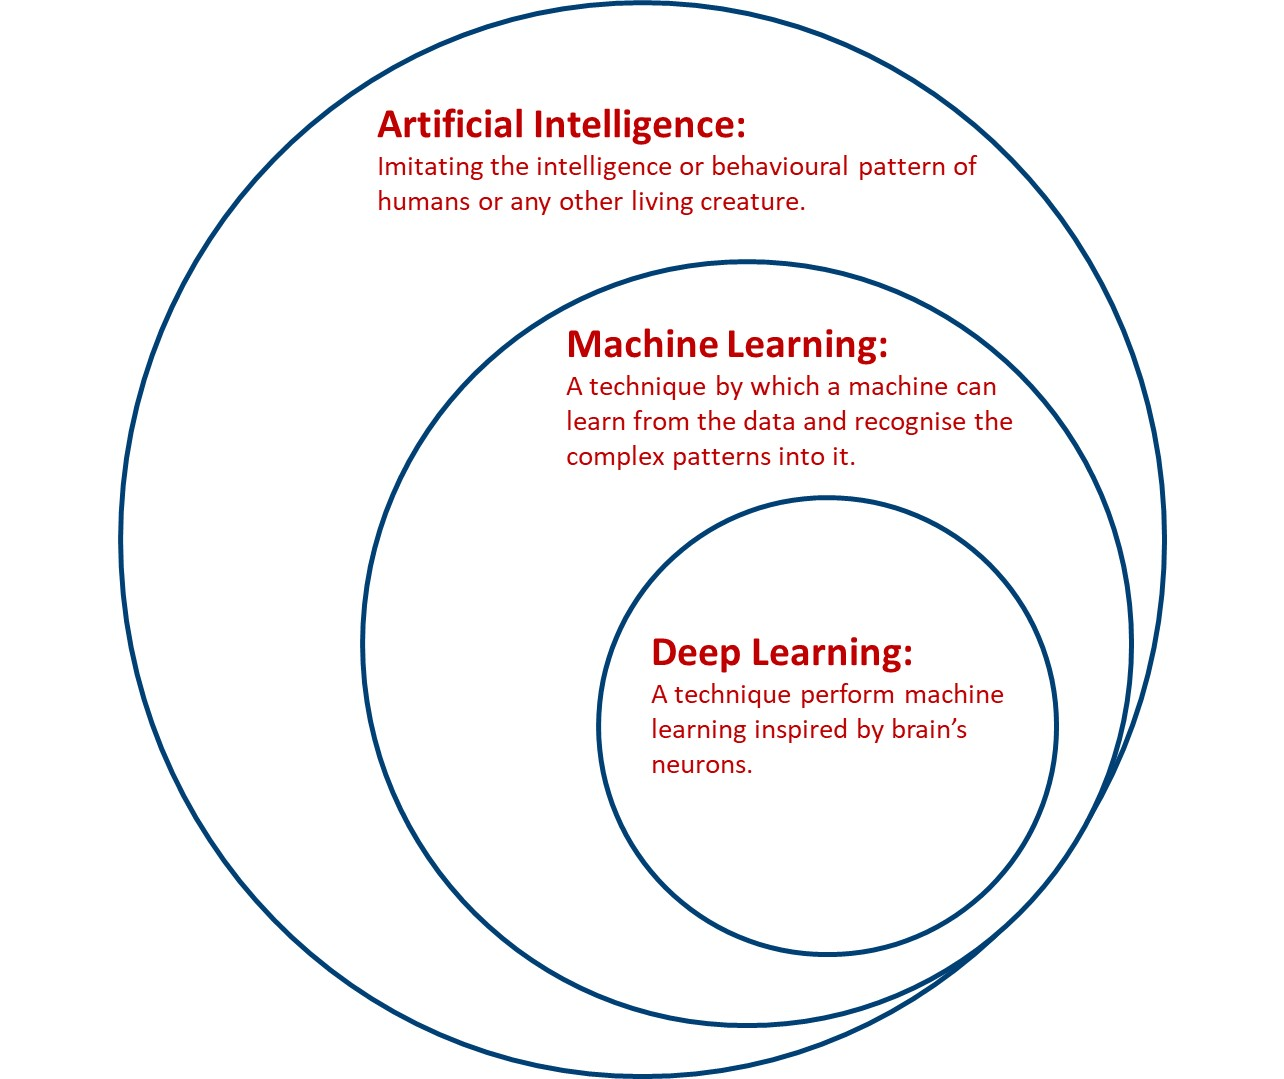
\includegraphics[scale=0.25]{images/Introduction/deeplearningsubset.jpg}
	    \caption[Relationship between Artificial Intelligence, Machine Learning, and Deep Learning.]{Relationship between Artificial Intelligence, Machine Learning, and Deep Learning.}
	    \label{fig:deepLearningSubset}
	    \end{center}
\end{figure}


The concept of deep learning was invented as early as the 1950s, although it was largely ignored until the 1980s and 1990s. However, with the efficient, fast computation hardware, and abundant data since decade it has become a popular research topic among many \ac{AI} research institutions, organizations, and startups. Deep learning is inspired by the biological network of neurons present inside the brain. Deep learning algorithms learn to discover meaningful, complex patterns in the digital representation of data, like sounds and images. To achieve this, deep learning uses a multi-layered structure of algorithms called Artificial Neural Networks (\acp{ANN}). \acp{ANN} are the heart of deep learning. They are flexible, efficient, and scalable, and suitable for vast and highly complex deep learning tasks like classifying billions of images (e.g., Google Images, Instagram, and Facebook), object detection (e.g., Tesla's Self-driving Cars), improving speech recognition systems (e.g., Apple's Siri, Amazon's Alexa, and Google Assistant), defense systems (Israel's Iron Dome, U.S.A's Patriot Missile System), and recommending the best videos to watch to hundreds of millions of users every day (e.g., YouTube).

Neural Networks are capable enough to solve complex problems by extracting features, recognizing patterns in data efficiently. However, there are certain challenges while training the neural networks. The two main things that can cause difficulties are bad algorithms and bad data. Let's start with some examples of bad data. Insufficient training data is one of the main problems that may arise when training deep learning models. A large amount of training data is required for most deep learning models to work properly. The second is the poor quality data. If the training data is wrong, noisy, and full of outliers, it will make it difficult for the model to detect patterns in the data. Hence the model will not perform well. The third is the irrelevant features. The model will only learn if the training data has more relevant features than irrelevant features. 

%Hence, it is often worth putting effort and spend time cleaning up training data. Most of the Machine Leaning Engineers spend significant amount of time doing the same. 

Now, that after some examples of bad data, let's look at some of the examples of bad algorithms. Overfitting and underfitting are one of the main problems of deep learning. ``Overfitting happens when the model is too complex relative to the amount and noisiness of the training data'' \cite{10.5555/3153997}. In the overfitting, model learns training data including noise to the extent, it negatively impacts the performance of the model, leading to higher generalization error on unseen data. One of methods used to decrease the risk of overfitting is regularization \cite{kukacka2017regularization}. Regularization is one of the solutions provided to generalize a model better to the new examples. ``Underfitting is the opposite of overfitting, it occurs when a model is too simple to learn the underlying structure of the data'' \cite{10.5555/3153997}. In the case of the underfitting model, it neither learns training data nor generalize to the unseen data. The problem of underfitting is resolved ``by choosing a powerful model with more parameters and providing better features during the model learning process'' \cite{10.5555/3153997}. The training of the deep learning model is highly influenced by the quality and quantity of the data that has been used for the training. But in many cases, data is scarce and it is very difficult to have data that is labeled and annotated.


%In the following sections, the motivation behind this thesis is discussed in section \ref{motivation} and the problem statement is discussed in section \ref{ProblemStatement}. The objectives of this thesis discussed in section \ref{thesisobjectives}. The thesis structure and limitations are discussed in section \ref{thesisstructurelimitations}. Finally, the terminologies used in this thesis are defined in section \ref{terminology}.



\section{Motivation}\label{motivation}

Deep learning methods have many effective applications in several fields, including natural language processing and computer vision. However, these methods still are limited by poor generalization due to the insufficient quantity of training data \cite{8978087}. Annotated data are scarce when it comes to developing deep learning models for computer vision applications. The performance of such deep learning models can be improved with the introduction of a large amount of annotated data. However, due to the high cost of data annotation, it is difficult to obtain a large set of annotated training data, especially when there are many classes of data. To overcome the obstacle of the scarcity of annotated data, there are some methods available to tackle this problem. The popular methods are Active Learning \cite{hemmer2020deal}, Data Augmentation \cite{Shorten.2019}, Transfer Learning \cite{zhuang2020comprehensive}, and Domain Adaptation \cite{redko2020survey}. 

\begin{figure}[H]
        \begin{center}
 	    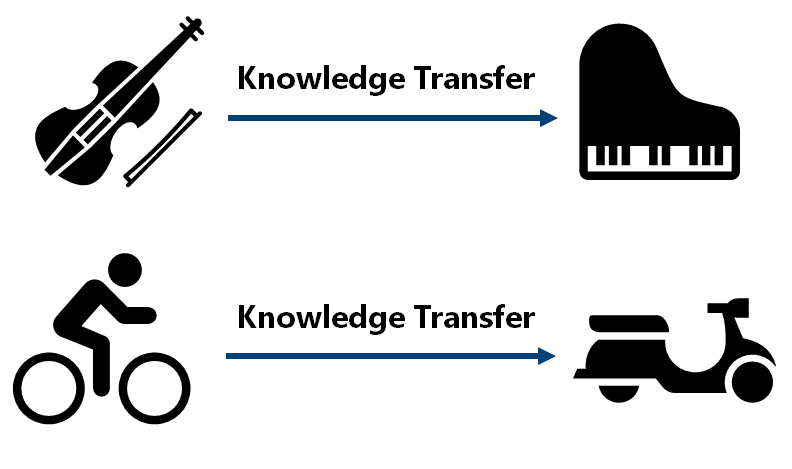
\includegraphics[scale=0.40]{images/Introduction/TransferLearning.png}
	    \caption[Simple examples of transfer learning.]{Simple examples of transfer learning.}
	    \label{fig:TransferLearning}
	    \end{center}
\end{figure}

This thesis aims to solve the data scarcity problem using the domain adaptation method. Domain adaptation is a subcategory of transfer learning in which the task is to transfer the knowledge from the source domain to the target domain. ``Transfer learning is the ability of a system to recognize and apply the knowledge learned from one task to another task'' \cite{zhuang2020comprehensive}. For example, if a person has mastered one musical instrument like the violin, can learn piano faster compared to others, as the knowledge of one musical instrument can be applied while learning another musical instrument. Figure \ref{fig:TransferLearning} shows an intuitive example of transfer learning. Transfer learning inspired by human behavior, humans beings are capable to transfer knowledge from one domain to another domain. The transfer learning grasps knowledge from the source domain to improve the learning performance in the target domain so the number of labeled samples required in the target domain can be reduced. It is important to mention, transfer learning is effective only if the source domain and target domain are related. For example, learning bicycles will not help to learn piano faster. Qiang Yang et al.\cite{5288526} have performed survey on transfer learning, more information about the transfer learning can found in their research paper.  

When the source and target domains are the same and learning tasks also the same, then such a learning problem becomes a traditional machine learning problem \cite{5288526}. When the source and target domains are different but related, and learning tasks are the same then, such a learning problem becomes a domain adaptation problem \cite{5288526}. In domain adaptation, source and target domains have the same feature space but different distributions in contrast to transfer learning, which includes cases where the target domain's feature space is different from the source domain's feature space \cite{5288526}. Domain adaptation is distinguished depending upon the similarity or dissimilarity of feature space and availability of annotated data in the source domain and target domains. The domain adaptation has two categories, if the feature space is the same between the source domain and target domain is called homogeneous domain adaptation. If the feature space is different between the source and target domain is called heterogeneous domain adaptation. Further homogeneous and heterogeneous domain adaptation divided into three types of domain adaptation, supervised domain adaptation, semi-supervised domain adaptation, and unsupervised domain adaptation. In the supervised domain adaptation, the samples in the target domains are labeled. Semi-supervised domain adaptation has a small set of labeled and unlabeled samples in the target domain. And, in unsupervised domain adaptation, the samples in the target domain are not labeled \cite{5288526}. A simple example of domain adaptation of  \ac{SVHN} transformed into Handwritten Digits shown in figure \ref{fig:DA}. The difference between traditional machine learning and domain adaptation is shown in figure \ref{fig:DomainAdaptation}.


\begin{figure}[H]
        \begin{center}
 	    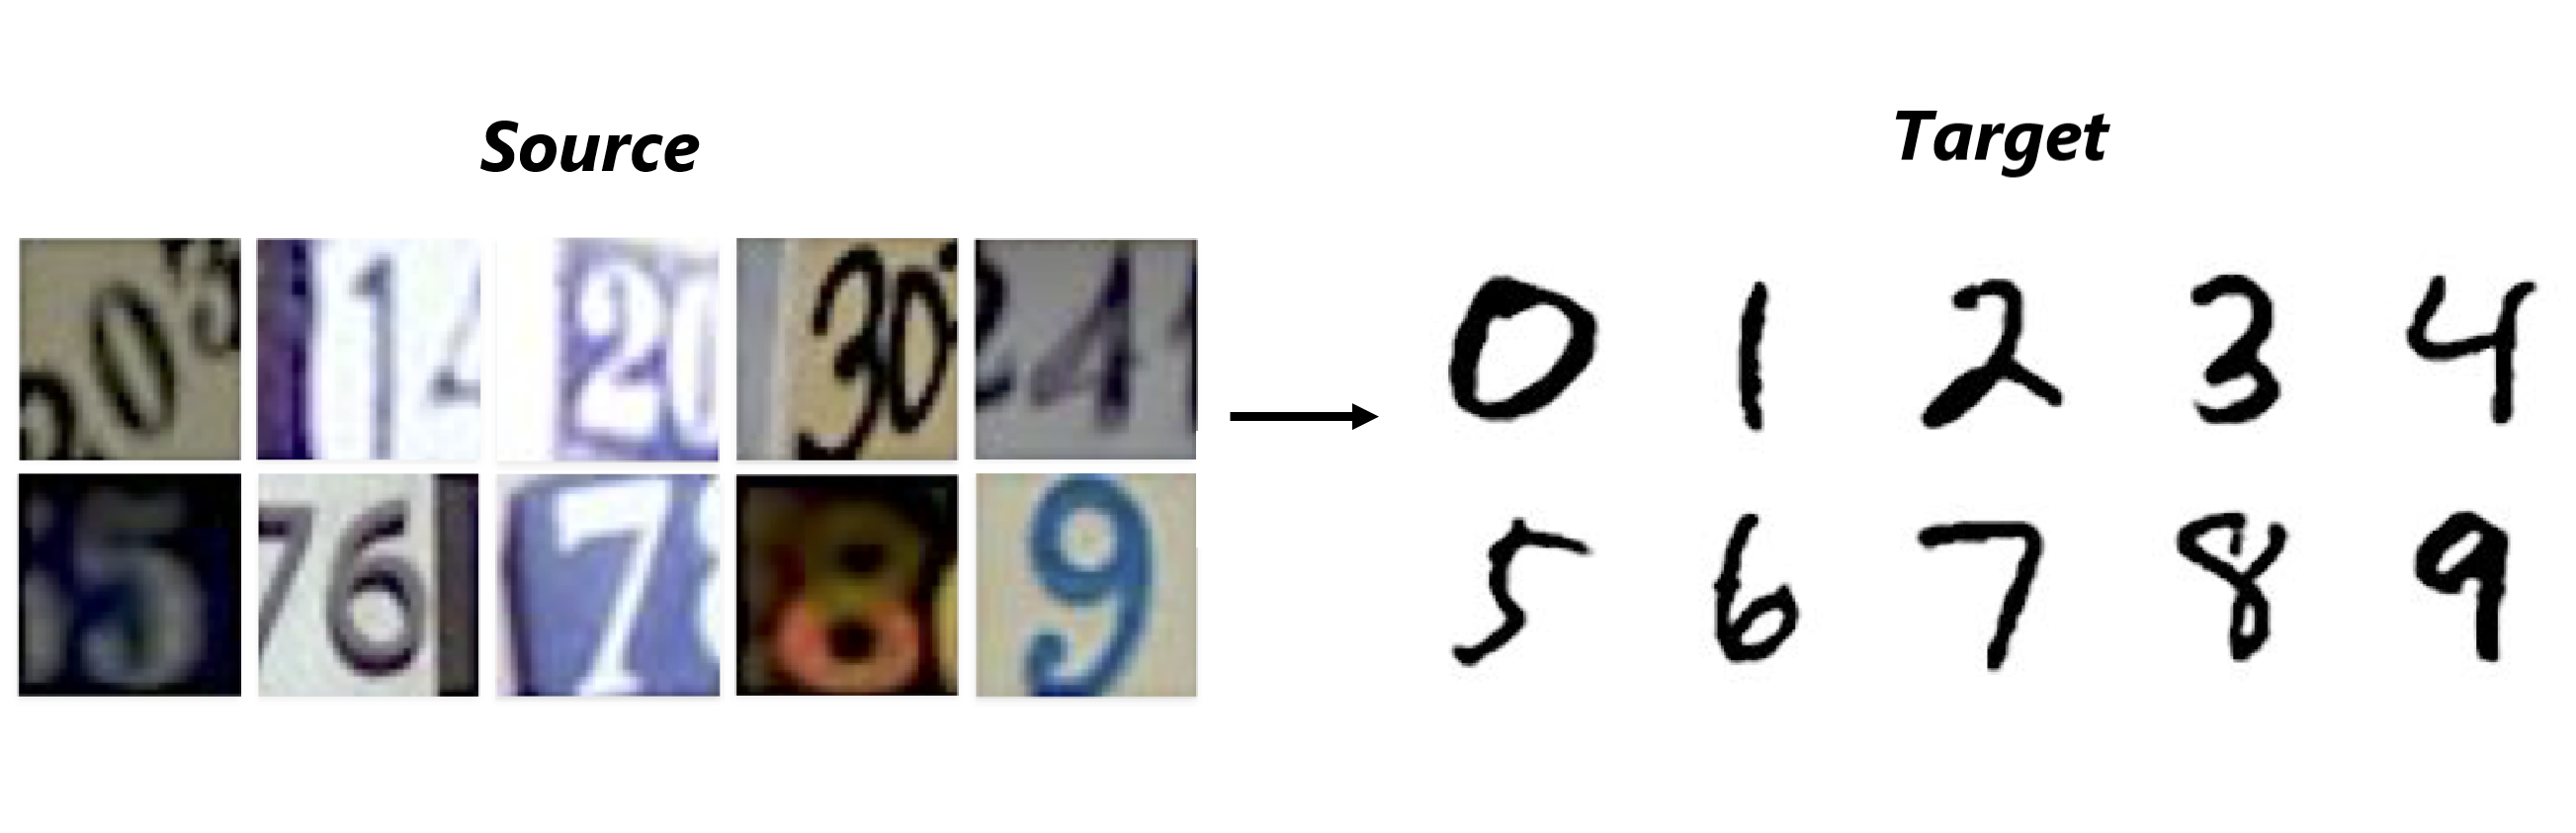
\includegraphics[scale=0.15]{images/Introduction/DA.png}
	    \caption[Simple example of domain adaptation from \ac{SVHN} dataset to \ac{MNIST} Dataset for the digit recognition task.]{Simple example of domain adaptation from \ac{SVHN} dataset \cite{37648} to \ac{MNIST} Dataset\footnotemark for the digit recognition task.\footnotemark}
	    \label{fig:DA}
	    \end{center}
\end{figure}
\footnotetext[1]{\url{http://yann.lecun.com/exdb/mnist/} last access: \dcdate}
\footnotetext[2]{\url{https://machinelearning.apple.com/research/bridging-the-domain-gap-for-neural-models} last access: \dcdate}





To understand how domain adaptation works, let's have a simple example. Consider the source domain represented by the \ac{SVHN} dataset. It is a collection of house number images, and the target domain represented by the \ac{MNIST} dataset, which is a collection of handwritten digit images.  When the \ac{CNN} is trained and evaluated on the source domain \ac{SVHN} dataset for the task of identifying numbers it will achieve good accuracy. However, the same classifier will perform worst when evaluated the\ac{MNIST} dataset. This performance gap occurs due to differences between the domain data distribution. The images in the \ac{SVHN} dataset consist of different fonts, blur, noise, and different backgrounds. But the images in the \ac{MNIST} dataset contain a clean background and handwritten strokes. Now consider images are scarce in the target domain. Only a small amount of the target domain images are available, which are unlabeled. As we know training a classifier using a smaller amount of data leads to underfitting and eventually leads to the worst performance on unseen data. Hence, to create a sufficient amount of data, the domain adaptation model is trained. It learns to transfer the underlying knowledge from the source domain to the target domain. In this case, labeled data is available in the source domain, and unlabeled data available in the target domain. Such a setup is called unsupervised domain adaptation because the model learns to transform images from one domain to another in the absence of labeled data in the target domain, and without taking much help from the labeled data from the source domain during the learning process. Using this domain adaptation model, large amount of annotated data can be created in the target domain by transforming source domain images into target domain images. Once a sufficient amount of images present in the target domain, the task to identify numbers in the target domain can be improved significantly. Nowadays, the domain adaptation technique is widely used in the field of \ac{HTR} \cite{Kang_2020}, Image Classification \cite{5288526}, Style Transfer \cite{johnson2016perceptual}, and \ac{OCR} \cite{8978011} to solve the problem of scarcity of data. Making such applications robust, accurate, and efficient is a big task, which requires years of research. The scope of this thesis is limited to improving document image classification using the proposed domain adaptation technique.

\begin{figure}[H]
        \begin{center}
	    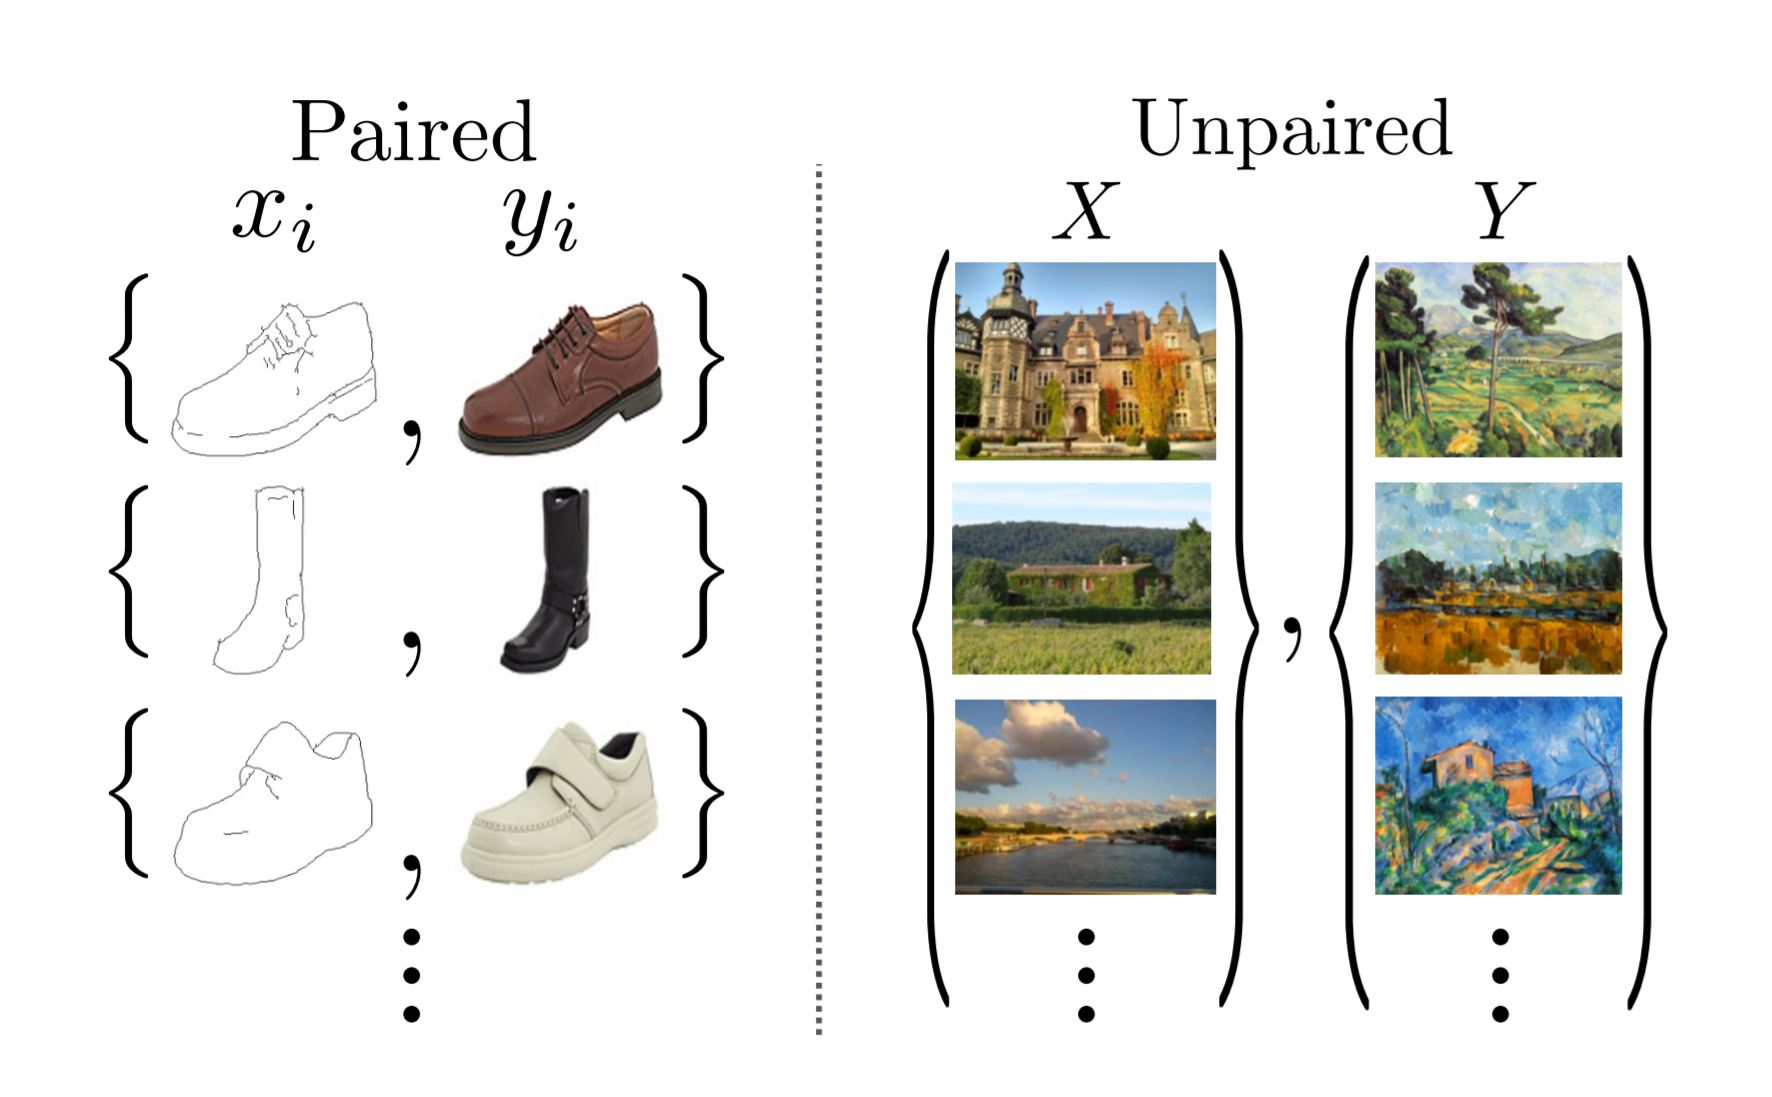
\includegraphics[scale=0.50]{images/Introduction/img_translation.JPG}
	    \caption[Examples of the paired training data set and the unpaired training data set.]{The paired training data set consists of training examples, in which there is a correspondence between the source domain and the target domain (Left, Edges \leftrightarrow Images). But in the unpaired training data set, there is no correspondence between the source domain and the target domain (Right, Photographs \leftrightarrow Painitings) \cite{zhu2020unpaired}.}
	    \label{fig:img_translation}
	    \end{center}
\end{figure}


\begin{figure}[H]
        \begin{center}
	 	    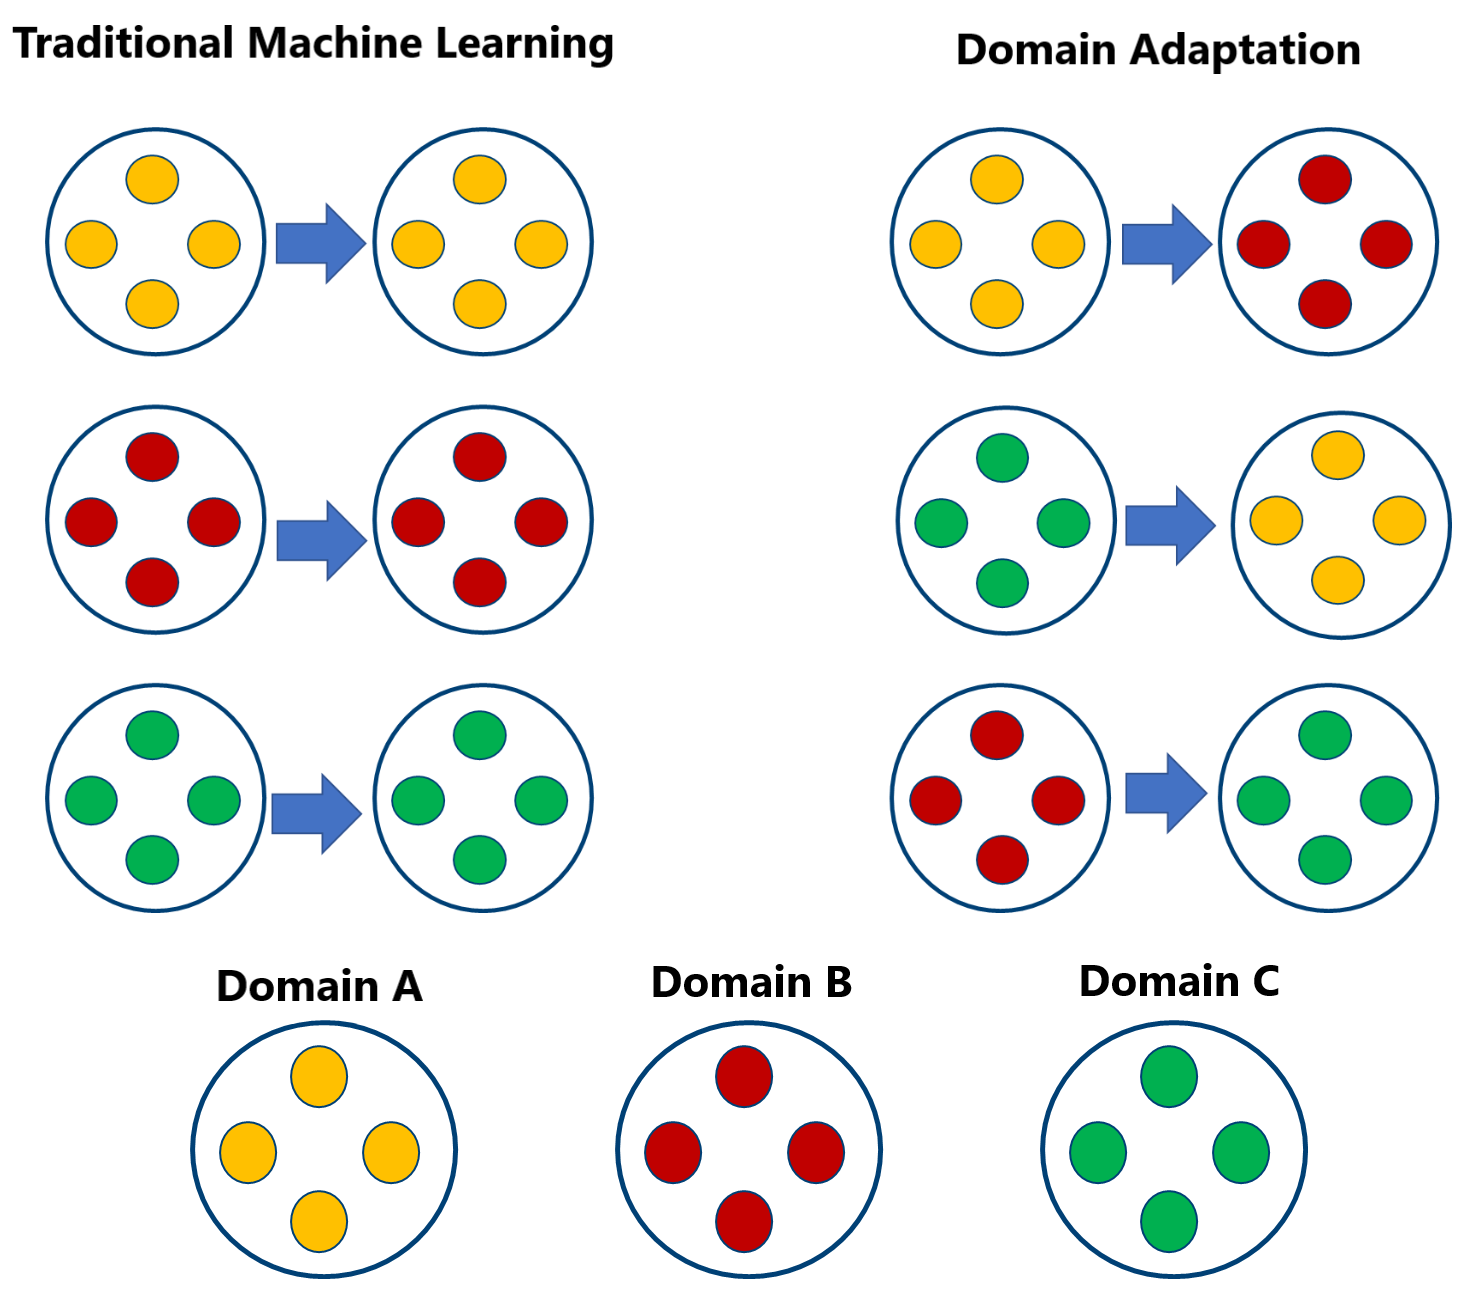
\includegraphics[scale=0.28]{images/Introduction/DomainAdaptation.png}
	    \caption[Difference between traditional machine learning and domain adaptation.]{Difference between traditional machine learning and domain adaptation.}
	    \label{fig:DomainAdaptation}
	    \end{center}
\end{figure}




\section{Problem Statement}\label{ProblemStatement}

As mentioned earlier, annotated data are scarce when it comes to the training of neural networks, and labeling a large set of data is a costly and tedious job. For example, real document images (figure \ref{fig:RealImage}) with different types of handwriting. In such cases, machine learning engineers have to inevitably generate synthetic data. However, deep learning models trained using synthetic data will not generalize well on real data \cite{8978087} (figure \ref{fig:Problem}). The synthetic data lacks realism \cite{8978087}. It does not possess a similar noise distribution as real data \cite{8978087}. Hence, in the last two decades, numerous domain adaptation methodologies have been introduced \cite{8978011}. Such methods are used to transform synthetic data into realistic data by reducing the divergence between the distribution of real data and the distribution of synthetic data. In this thesis, a domain adaptation application is developed using \ac{CycleGAN} \cite{zhu2020unpaired} to reduce the domain gap between synthetic data distribution and real data distribution. The \ac{CycleGAN} is an extended variant of Generative Adversarial Network (\ac{GAN}) \cite{goodfellow2014generative}. 

This application is designed in consultation with, \ac{ML} developers at Elevait Deutschland GmbH, a Germany-based company that develops \ac{AI} applications for business use-cases. Elevait is widely contributing in the field of Cognitive Business Robotics \cite{Metta2012} to automate document processing. Elevait has developed state-of-the-art \ac{HTR} and \ac{OCR} tools to process documents and extract information from documents. To make those systems robust and efficient a large number of document images are required. The idea is to create a large number of synthetic document images to have a large quantity of annotated data. However, the synthetic document images will not generalize well when they have to process real document images because the real document images have different noise distribution. Furthermore, artifacts such as salt-and-pepper, background noise, blur due to camera motion or shake, watermarks, stains, wrinkles, and fading text are often introduced during the scanning process. Hence this application is used to transform synthetic document images into realistic document images. This application is capable to capture the noise distribution of real documents and transform an image from the source domain to the target domain. Such a kind of transformation is called image-to-image translation.


\begin{figure}[H]
        \begin{center}
	    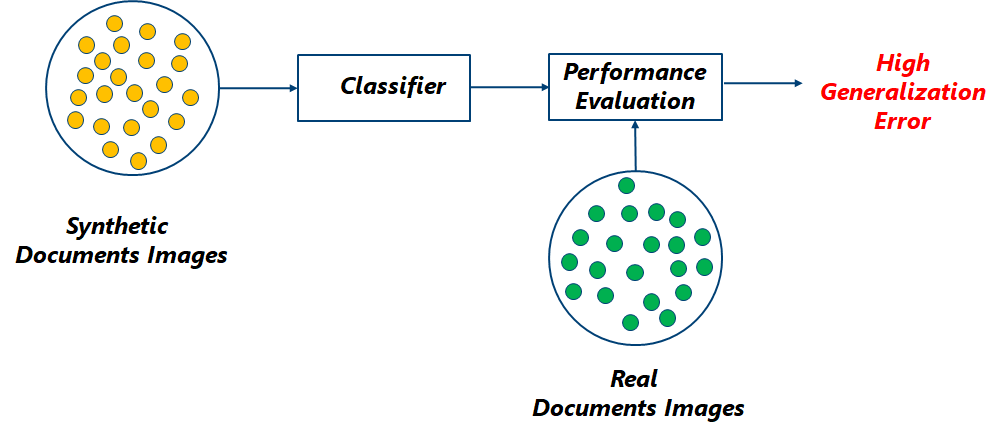
\includegraphics[scale=0.60]{images/Introduction/Problem.png}
	    \caption[An illustration of the problem to be solved in this thesis.]{An illustration of the problem to be solved in this thesis.}
	    \label{fig:Problem}
	    \end{center}
\end{figure}


The synthetic document images are created using templates (figure \ref{fig:template}) and handwritten crops (figure \ref{fig:keinwifi}) retrieved from handwriting datasets like \ac{MNIST} (figure \ref{fig:handwrittenCrops}) or any other datasets. These templates contain fields like are customer number, customer name, and other customer information. These fields are represented by using bounding boxes. The bounding boxes are annotated using \ac{COCO} annotations \cite{10.1007/978-3-319-10602-1_48}. In this thesis, the handwritten crops are inserted over the templates to generate numerous synthetic document images. As mentioned earlier deep learning models trained using synthetic document images will not generalize well on real document images. In this thesis, the handwritten crops are inserted over the templates to generate numerous synthetic document images. As mentioned earlier deep learning models trained using synthetic document images will not generalize well on real document images. Further, the image-to-image translation application is developed using \ac{CycleGAN} to transform synthetic document images into realistic document images. ultimately, to reduce the domain gap between synthetic data distribution and real data distribution. 


A large number of realistic document images can be generated to tackle the problem of data scarcity in the target domain. As we already know that real document images are scarce and labeling images is a tedious and costly job. Our image-to-image translation application transforms synthetic document images to realistic document images to solve the following problems. First, We have labeled synthetic document images in the source domain, ultimately we get labeled, transformed realistic document images in the target domain. So the problem of labeling, annotations, and scarcity is solved. Second, Consider we have a huge chunk of real document images which are not labeled. If the simple classifier is trained on realistic document images. Later, these chuck of real document images can be automatically classified with ease. This will save data annotation and data collection efforts. Further, making image classification tools in the target domain robust and efficient even in the absence of real data. 

The figure \ref{fig:Problem} describes if the classifier is trained using synthetic document images, it won't generalize well on the unseen real document images. Further, it leads to high generalization error, hence represented in dark red color for better understanding. In figure \ref{fig:ProposedSolution} Data distribution in light green color represents realistic data which is generated by the domain adaptation method. Dark green represents the real data. The proposed solution is to use domain adaptation methods like the image-to-image translation to reduce the divergence between data distributions. Further, the classifier is trained using realistic document images, it generalizes better on the unseen real document images compared to the classifier are trained using synthetic document images, hence low generalization error represented in light red color for better understanding compared to figure \ref{fig:Problem}.


\begin{figure}[H]
        \begin{center}
	    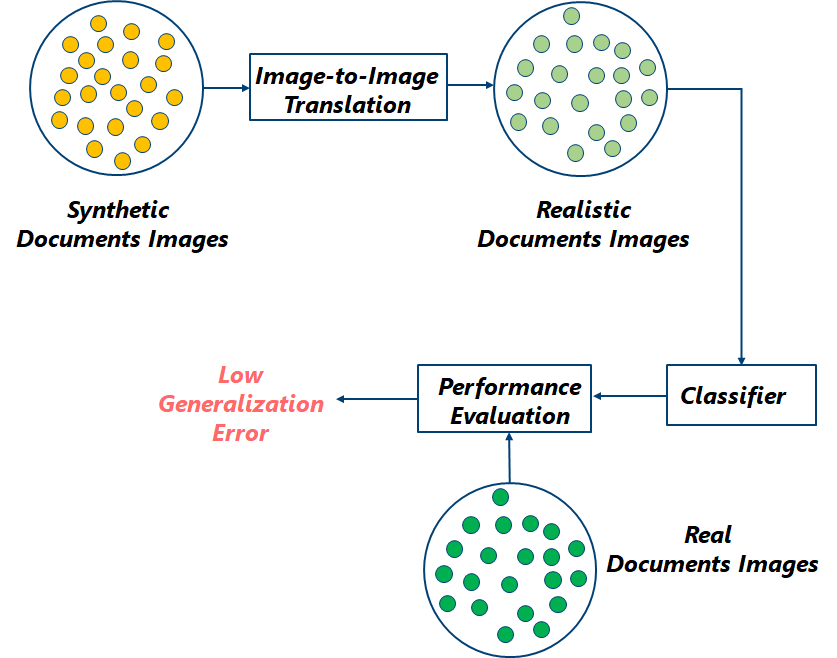
\includegraphics[scale=0.55]{images/Introduction/ProposedSolution.png}
	    \caption[Illustration of the solution proposed to reduce the domain gap between the synthetic document images and the real document images.]{Illustration of the solution proposed to reduce the domain gap between the synthetic document images and the real document images.}
	    \label{fig:ProposedSolution}
	    \end{center}
\end{figure}

\newpage

\section{Thesis Objectives}\label{thesisobjectives}
Every research work has its own objectives. The purpose of this thesis to close domain gap between synthetic data distribution and real data distribution by developing an image-to-image translation application using \ac{CycleGAN}. The developed image-to-image translator is used to transform synthetic document images into realistic document images. In addition, in this thesis, experiments are conducted to understand the domain gap between data distributions. The objectives of this thesis are listed below:

\begin{itemize}[label=\EightFlowerPetalRemoved]
 \item Objective 1 is to conduct a literature survey, in which different types of image-to-image translation methods should be discussed and explained in related work. In addition, it is necessary to propose a theoretical comparison between existing methods, which ultimately leads to the decision to adopt a specific method to solve the reasons for the problem statement of the thesis.
\item Objective 2 is to create and collect source and target domain datasets to train the proposed image-to-image translation application. In addition, a test dataset of annotated real images is also collected for evaluation.
\item Objective 3 is to design, implement, and train image-to-image translation application.
\item Objective 4 is to perform experiments, to determine the quality of images generated by the image-to-image translation application. In addition, train classifiers on different data distribution and evaluate them on real data, to analyze the domain gap between those distributions and real data distribution.
\item Objective 5 is to document all the information regarding the thesis, for example, related works, selected methodology, fundamentals required to understand the work, experiments, results, limitations, conclusion, and future work.
\end{itemize}


\section{Thesis Limitations and Structure}\label{thesisstructurelimitations}
The domain adaptation field is promoting incremental findings, hence this thesis has its limitations due to time deadlines. The proposed image-to-image application is implemented only using \acp{CycleGAN}. The implementation in and comparison with other methodologies are placed apart for future work. The scope of this thesis is limited to the improvement of real document images classification by increasing the quality and quantity of labeled data in the target domain, and reducing the domain gap between synthetic data distribution and real data distribution. The rest of this thesis is organized as follows. Chapter \ref{relatedworks} briefly reviews literature of numerous \acp{GAN} variants and existing methods. Chapter \ref{fundamentals} discusses the about \acp{GAN} and Convolution Neural Networks (CNNs) to develop fundamental knowledge to understand this thesis. The proposed approach is described in chapter \ref{methodology} along with the objective function and algorithm. The implementation of the proposed solution, dataset details, and neural networks architectures, and training details are described in chapter \ref{implementation}. The experiments and results are presented in chapter \ref{evaluation}. Finally, this work has been concluded in Chapter \ref{conclusion} along with the future work and the limitations.


\section{Terminology}\label{terminology}

In this thesis for simplicity and readability, many terms are explained beforehand for better understanding and to avoid confusion. The following terms described in this thesis are consistently used throughout this thesis. The term ``Artificial Neural Networks'' will be used as ``Neural Networks'' interchangeably. The images generated by the \ac{CycleGAN} generator in the target domain are called ``Realistic Document Images'' and they are also interchangeably called ``\ac{CycleGAN} Generated Document Images''.
So, the distribution of ``\ac{CycleGAN} Generated Document Images'' is called ``\ac{CycleGAN} Generated Data Distribution''.













%%%%%%%%%%%%%%%%%%%%%%%%%%%%%%%%%%%%%%%%%%%%%%%%%%%%%%%%%%%%%%%%%%%%%%%%%%%%%%%%%%%%%%%%%%%%%%%%%%%%%%%%%%%%%%%%%
%The handwriting datasets and document images datasets are can not be disclosed or cited due to data privacy concerns and copyright issues.
%By comparing a classifier performance on real data distribution by first training them on data distributions like synthetic data, faxified data, and \ac{CycleGAN} generated data. 


%Every research work comes with definite objectives to achieve. The Objective 1 of the thesis is to perform a literature survey, in which, different types of image-to-image translation methods should be discussed. Furthermore, the theoretical comparison between existing methods must be discussed, to finally decide a methodology to solve the problem statement. Objective 2 is to create and collect datasets to train neural networks by keeping small testing aside to evaluate models. Objective 3 is to proceed with the design and development of the neural networks during the implementation phase of this thesis. Objective 4 is to perform experiments, and Objective 5 is to analyze, evaluate results achieved by the chosen method, implementation. Objective 6 is to document all the information regarding the thesis, for example, chosen methodology, fundamentals required to understand the work, experiments, results, limitations, conclusion, and future work.


%during the implementation phase of this thesis. In this step the \ac{CycleGAN} is implemented and trained.

\begin{comment}
The neural networks trained in this thesis using images of resolution $256 \times 256$. In the real world, document images are of higher resolution.
\end{comment}

\begin{comment}
The \ac{CycleGAN} is used to transform synthetic document images into realistic document images as \acp{CycleGAN} is the state-of-the-art for unpaired image-to-image translation. This image-to-image translation application deals with synthetically generated document images, which are created using empty template images and handwritten crops retrieved from data sets like \ac{MNIST} or any other data sets. The dataset used in the thesis is copyrighted, which can not be exposed to public use. Handwritten crops are pasted over the empty template images to generate numerous synthetic document images. Nevertheless, deep learning models trained using synthetic document images will not generalise well on real document images. Hence, the \ac{CycleGAN} is used to perform the unpaired image-to-image translation and transform synthetic document images into realistic document images.
\end{comment}




\begin{comment}
This thesis starts with Objective 1, Literature Survey, in which, different types of image-to-image
translation methods are discussed. Also, it addresses how general GANs are extended by modifying
their objective function to solve different kinds of image-to-image translation problems. General
GANs suffers from mode collapse, literature survey helped to find the efficient and easy solution
to overcome such problems. Furthermore, the theoretical comparison between existing methods
has discussed, ultimately deciding a methodology to solve the problem statement. Objective 2,
the creation of datasets is an important aspect of training any neural network. The datasets for
synthetic document images, faxified document images have been created. Also, a large chunk of
unlabeled real document images is collected. A small testing dataset of real document images is
kept aside to evaluate models. Objective 3, once the dataset was ready, the software development
was carried out during the implementation phase of this thesis. Objectives 4 and 5, experiments
were performed to analyze whether the chosen method, implementation, and approach produced
acceptable results, and all the results were recorded for evaluation. Objective 6, was the challenging
phase, all the information regarding this thesis, for example, chosen methodology, fundamentals
required to understand the work, results, and conclusion of the thesis has been written in a report
for submission.
\end{comment}


\begin{comment}
The architecture of \ac{CycleGAN} is adapted from Johnson et al. ~\cite{johnson2016perceptual}. The generator network is implemented using a sequence of downsampling convolutional blocks to encode the $256 \times 256 \times 1$ grayscale input image, 9 \ac{ResNet} convolutional blocks to transform the image, and a number of upsampling convolutional blocks to generate the output image of the same dimension as the input image. The reason behind using residual blocks is it resolves the vanishing gradient problem in deep neural networks. The discriminator networks uses PatchGAN ~\cite{isola2018imagetoimage}. In PatchGAN, after feeding one input image to the network, it gives you the probabilities of two things: either real or fake, but not in scalar output indeed, it used the $N \times N$ output vector. Here $N \times N$ can be different depending on the dimension of an input image. The architecture of both generator and discriminator networks will be thoroughly discussed in Chapter \ref{implementation}. To evaluate the quality of images generated by the \ac{CycleGAN}, a classifier is trained on the \ac{CycleGAN} generated data and its accuracy on a real test set is used as a metric to measure how well the \ac{CycleGAN} model distribution matches the real data distribution. Basically, The classification capability of the trained classifier is used as an objective measure to assess the quality of images generated by \ac{CycleGAN}. 
\end{comment}







\begin{comment}
\begin{figure}[H]
        \begin{center}
	    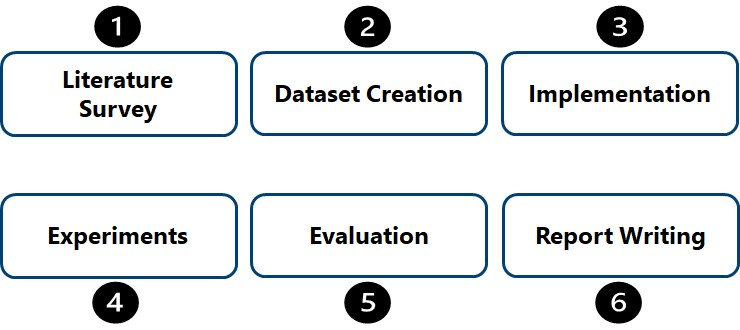
\includegraphics[scale=0.50]{images/ThesisObjectives2.JPG}
	    \caption{Thesis Objectives.}
	    \label{fig:ThesisObjectives}
	    \end{center}
\end{figure}

\end{comment}

